\documentclass[dvipsnames, article, a4paper, oneside, 12pt]{memoir}
\newsubfloat{figure}
\linespread{1.25}
\setlength{\parskip}{1em}
\setlength{\parindent}{0em}

\usepackage[]{mathtools}
\usepackage[]{amssymb}
%\usepackage[]{libertine}
%\usepackage[]{libertinust1math}
\usepackage[]{mathpazo}
\usepackage[]{eulervm}
\usepackage[T1]{fontenc}
\usepackage[]{microtype}
\usepackage[]{geometry}
\usepackage[]{amsthm}
\usepackage[]{thmtools}
\usepackage[usedvipsnames]{xcolor}
\usepackage[]{bm}
\usepackage[]{amsmath}
\usepackage[]{commath}
\usepackage[]{todonotes}
\usepackage[]{graphicx}
\usepackage{titling}
\usepackage{mdframed}
\usepackage[]{FiraMono}
\usepackage[]{FiraSans}
\usepackage[]{siunitx}

\usepackage[backend=biber, style=alphabetic, url=false, doi=false]{biblatex}
\addbibresource{../../FYS-STK4155.bib}
\usepackage[noabbrev, capitalize]{cleveref}


\declaretheorem[style=remark, name=Remark,
mdframed={
}]{remark}
\declaretheorem[style=remark, name=Assumption,
mdframed={
}]{assumption}

\title{\Large\textsc{Regression And Resampling Techniques \\
  FYS-STK4155 \\
Assignment One}}
\author{Ivar Haugal{\o}kken Stangeby}

\newcommand{\x}{\bm{x}}
\newcommand{\C}{\mathbb{C}}
\newcommand{\X}{\bm{X}}
\newcommand{\diag}[1]{\mathrm{diag}(#1)}
\newcommand{\MSE}[1]{\mathrm{MSE}(#1)}
\newcommand{\R}[1]{\mathrm{R}^2(#1)}
\newcommand{\expect}{\mathbb{E}}
\DeclareMathOperator{\var}{Var}
\DeclareMathOperator{\cov}{Cov}
\newcommand{\OLS}{\mathrm{OLS}}
\DeclareMathOperator{\SD}{SD}
\newcommand{\ridge}{\mathrm{ridge}}
\newcommand{\lasso}{\mathrm{lasso}}
\newcommand{\python}{\textsf{Python}{}}
\newcommand{\sgn}{\,\mathrm{sign}{}}

\newcommand{\mat}[1]{\bm{#1}}
\newcommand{\y}{\bm{y}}
\newcommand{\data}{\bm{\Omega}}
\newcommand{\cost}{\mathcal{C}}
\newcommand{\N}{\mathcal{N}}
\newcommand{\basis}{\mathcal{B}}
%\newcommand{\set}[1]{\left\{\, #1 \right\}}

\pretitle{%
  \begin{center}
    
\includegraphics[scale=0.7]{images/franke_shadow.pdf}\\[\bigskipamount]
}
\posttitle{\end{center}}

\begin{document}
  \maketitle 
  \clearpage
 	
  \begin{abstract}
	  In this project, we implement and compare three different variants of
	  linear regression. Namely, ordinary least squares (OLS), Ridge
	  regression, and Lasso regression. We test the methods on terrain data
	  taken from a region near Stavanger, Norway. Initial implementation
	  tests are done on an artificial data-set based on noisy samples of
	  the Franke function. Statistical quantities pertaining to the various
	  model functions are computed and compared. We also give an
	  introduction to the theory and motivation behind the three methods.
  \end{abstract}

  \tableofcontents

  \chapter{Introduction}
   
  Regression analysis is the act of estimating relationships among variables.
  In this project, we study various regression methods in more detail. In
  particular, we compare the \emph{ordinary least squares} (OLS) method with
  the \emph{Ridge regression} and \emph{Lasso regression} techniques. As we
  shall see, these three methods are all variations over the same theme. We
  start by testing the methods on noisy data sampled from a function known as
  \emph{Franke's} bivariate test function (visualized on the title page), which
  has been in widespread use in the evaluation of interpolation and data
  fitting techniques. Finally, we run regression on real terrain data,
  comparing the aforementioned methods.

  \chapter{Regression Techniques}
  \label{chp:regression}

  In general, the goal of regression analysis is to fit a \emph{model function}
  \( f(\x, \beta) \) to a set of \( n \) data points \( \data = (\x_i,
  y_i)_{i=1}^n \). A simple example is that of a linear polynomial with two
  parameters:
  \begin{equation}
    f(x, \beta) = \beta_0 + \beta_1 x.
  \end{equation}
  The \emph{model parameters} \( \beta \) are determined in order to minimize a
  suitable \emph{cost function} \(\cost(\data, \beta)\) which measures to which
  extent the model function manages to capture trends in the data \( \data \).
  It is the choice of cost function \( \mathcal{C}(\data, \beta)\) which
  distinguishes  the three regression techniques, OLS, Lasso regression, and
  Ridge regression.

  \begin{assumption}
    \label{as:general_linear}
    It is often assumed a priori that the data is infact generated from a noisy
    model, such that each \( y_i \) can be described as
    \begin{equation}
      y_i = f(\x_i) + \varepsilon_i
    \end{equation}
    where each \( \varepsilon_i \sim \N(0, \sigma^2) \) is normally distributed
    with zero mean and variance \( \sigma^2 \). This assumption on the error
    gives rise to what is known as \emph{general linear models}.
  \end{assumption}


  \paragraph{The design matrix.} We are often interested in finding the best
  model function in a specific function space.  Assuming this space has a basis
  \( \basis = \set{\varphi_i}_{i=1}^M\), we may write our model function in
  terms of the basis functions and the model parameters as
  \begin{equation}
    \label{eq:gen_lin_mod}
    f(\x, \beta) \coloneqq \sum_{i = 1}^M \beta_i\varphi_i(\x).
  \end{equation}
  As an example, if we were to use the space \( \Pi_2^2 \) of bi-quadratic
  polynomials, our basis functions would be
  \begin{equation}
    \basis = \set{1, x, x^2, y, y^2, xy}.
  \end{equation}
  With this formulation, we can represent the approximation \( \hat{\y} \) to
  \( \y \) as a matrix product 
  \begin{equation}
    \label{eq:matrix_prod}
    \hat{\y} = \X\beta
  \end{equation}
  where \( \X \) is the \emph{design matrix} defined by components \(\X_{ij} =
  \varphi_j(\x_i)\), and \( \beta = [\beta_1, \ldots, \beta_M] \) is the model
  parameters. 

  \paragraph{Performance metrics.}
  In order to evaluate the how accurately the model function \( f(\data, \beta)
  \) captures trends in the target data \( \y \), a few standard performance
  metrics are  used.  Firstly, the \emph{mean squared error}:
  \begin{equation}
    \MSE{\y, \hat{\y}} \coloneqq \frac{1}{n} \sum_{i=1}^n (y_i - \hat{y}_i)^2
  \end{equation}
  which simply averages the squared error over all samples and estimates.
  Secondly, we have the \emph{coefficient of determination} or
  \emph{\(R^2\)-score}:
  \begin{equation}
    \R{\y, \hat{y}} \coloneqq 1 - \frac{\sum_{i=1}^n (y_i -
    \hat{y}_i)^2}{\sum_{i=1}^n (y_i - \overline{y})^2}.
  \end{equation}
  The \(R^2\)-score measures much of the variation in \( \y \) which can be
  attributed to a simple linear relation between \( \x \) and \( \y \). It is a
  ratio, thus a value of one tells us that all the variation in the data can be
  attributed to an approximate linear relationship between the data \(\x\) and
  the response variable \( \y \). A value of zero indicates that a non-linear
  model may be preferrable.
  

  \section{Ordinary Least Squares}
  
  One common cost function is the one which involves the sum of squared
  residuals (or squared errors):
  \begin{equation}
    \label{eq:mse}
    \cost_\OLS(\data, \beta) = \frac{1}{n}\sum_{i = 1}^n \varepsilon_i^2 \coloneqq \frac{1}{n}\sum_{i=1}^n (y_i - \hat{y}_i)^2
  \end{equation}
  where \( \hat{y}_i \coloneqq f(\x_i, \beta) \). The method involving the
  minimization of this specific cost function is known as \emph{least squares}.
  With the matrix notation from above in mind, we can also write the cost
  function as
  \begin{equation}
    \cost_\OLS(\data, \beta) = \frac{1}{n} (\y - \hat{\y})^T (\y - \hat{\y}).
  \end{equation}

  

  \subsection{Optimizing the parameters in OLS.}
  
  Assume now that our model is of the form given in \cref{eq:gen_lin_mod} and
  that our cost function is the mean squared error defined in \cref{eq:mse}. We
  are interested in finding the parameters \( \beta \) that minimize the cost
  function \( \cost(\data, \beta) \). Since \( \cost(\data, \beta) \) is
  convex, it suffices to differentiate with respect to \( \beta \) and equating
  to zero. 
  
  We have that
  \begin{align}
    \dpd{\cost_\OLS(\data, \beta)}{\beta} = \X^T(\y - \X\beta), 
  \end{align}
  and equating this to zero yields the familiar \emph{normal equations}
  \begin{equation}
    \X^T \y = \X^T\X\beta.
  \end{equation}
  If the matrix \( \X^T\X \) is invertible, we may obtain the solution by
  direct numerical matrix inversion. In this case, the optimal model parameters
  are found directly by
  \begin{equation}
    \label{eq:optimal}
    \beta_{\OLS} = (\X^T\X)^{-1}\X^T\y.
  \end{equation}
  However, these matrices may be ill-conditioned when the number of equations
  are very large, and it is therefore common to apply approximate solvers for
  the inverse, for instance using low-rank approximation based on
  \textsc{SVD}-decomposition, which we will briefly turn to in the following.

  \subsection{Singular value decomposition.}
  
  Recall that any matrix \( \mat{A} \in \C^{n, m} \) can be decomposed as
  \begin{equation}
    \mat{A} = \mat{U} \mat{\Sigma}\mat{V}^T,
  \end{equation}
  where \( \mat{U} \) and \( \mat{V} \) are comprised of the eigenvectors of \(
  \mat{A}\mat{A}^T \) and \( \mat{A}^T\mat{A} \) respectively. As these
  eigenvectors are orthonormal, it follows that both \( \mat{U} \) and \(
  \mat{V} \) are unitary matrices. Furthermore, \( \mat{\Sigma} \) is a matrix 
  \begin{equation}
    \mat{\Sigma} = \begin{bmatrix}
      \Sigma_1 & 0 \\
       0 & 0
    \end{bmatrix},
  \end{equation}
  where \( \Sigma_1 \) is a square diagonal matrix of size \( r \times r \)
  with the non-zero singular values of \( \mat{A} \). The integer \( r \) is
  the \emph{rank} of \( \mat{A} \). As the matrix \( \Sigma \) is mostly
  containing zeros, the information stored in \( \mat{A} \) is attributed to
  only some parts of \( \mat{U} \) and \( \mat{V} \). We can remove the
  redundant parts, and more compactly express \( \mat{A} \) as \( \mat{A} =
  \mat{U}_1 \mat{\Sigma}_1 \mat{V}_1^T \) without loss of accuracy in the
  decomposition. Here, \( \mat{U}_1 \) is \( m \times r \) and \( \mat{V}_1 \)
  is \( n \times r \).

  Applying the singular value decomposition to the matrix \(\X = \mat{U}
  \mat{\Sigma} \mat{V}^T\) we can analyze the expression for the prediction \( \hat{\y} \)
  in terms of the matrix \( \X^T \X \).  First of all, we have that
  \begin{align}
    \begin{split}
    \X^T \X &= \mat{V}\mat{\Sigma}^T\mat{U}^T\mat{U}\mat{\Sigma} \mat{V}^T\\
            &= \mat{V}\mat{D}\mat{V}^T, 
    \end{split}
  \end{align}
  where we have used that \( \mat{U}\mat{U}^T = \mat{I} \) and defined \(
  \mat{D} = \diag{\sigma_1^2, \ldots, \sigma_n^2} \).  Thus, plugging this into
  \cref{eq:optimal,eq:matrix_prod}, we obtain the expression
  \begin{align}
    \begin{split}
      \hat{\y} = \X \beta = \X (\mat{V}\mat{D}\mat{V}^T)^{-1} \mat{X}^T \y.
    \end{split}
  \end{align}
  Finally, substituting \( \X = \mat{U}\mat{\Sigma}\mat{V}^T \) and noting that
  diagonal matrices always commute, we end up with
  \begin{align}
    \begin{split}
      \hat{\y} = \mat{U}\mat{U}^T \mat{y}.
    \end{split}
  \end{align}

  \subsection{The bias-variance tradeoff} 
  \label{sub:bias_variance} 
  Since we are attempting to estimate a true distribution based on finite
  samples, there are certain statistical properties it is worthwile discussing.
  We follow the derivation from \autocite{mehtaHighbiasLowvarianceIntroduction2019}.  Recall
  \cref{as:general_linear} which states that our true data is generated from a
  noisy model
  \begin{equation}
    y = f(\x) + \varepsilon
  \end{equation}
  with \( \varepsilon \sim \N(0, \sigma^2) \).  We select a finite sample from
  the true data, which constitutes our finite data-set \( \data \).
  Furthermore, we have a model function \( f(\data, \beta) \) which depends on
  the selected data-set and the model parameters \( \beta \). Thus, our
  cost-function \( \cost \) will depend on the specific sample taken from the
  true distribution. It is of interest to examine the expected out-of-sample
  error \( \expect_{\data, \varepsilon}[\cost(\data, \beta)] \) of the model
  function over the sampled data set \( \data \) and the noise \( \varepsilon
  \). This can be decomposed into three distinct parts,
  \emph{\textcolor{Maroon}{variance}}, \emph{\textcolor{Blue}{bias}}, and
  \emph{\textcolor{Green}{noise}}:
  \begin{equation}
    \label{eq:bias_variance}
    \expect_{\data, \varepsilon}[\cost(\data, \beta)] = \frac{1}{n} \textcolor{Blue}{\sum_{i=1}^n \left(f(\x_i) - \expect_{\data}\left[\hat{y}_i\right]\right)^2}  + \frac{1}{n}\textcolor{Maroon}{\sum_{i=1}^n \expect_{\data}\big[\left(\hat{y}_i - \expect_{\data} [\hat{y}_i]\right)^2\big]} + \textcolor{Green} \sigma^2.
  \end{equation}
  See \cref{ap:derivation} for the full derivation. The bias-term measures the
  deviation of the expectation of the model function \(f(\data, \beta)\) from
  the true value \( f \), while the variance-term measures the fluctuations
  arising due to using different samples of the true data.
  
  Now, note that the equation above suggests that we should minimize both the
  variance and the bias of the model, in order to obtain the smallest
  generalization error of the model function. The variance term will be larger
  for complex models, as performing a fit on one sampled data-set will not
  neccessarily translate well to another sampled data-set. The bias term
  measures errors introduced by making certain assumptions about the relations
  between the covariates \( \X \) and the response \( \y \). In our case, we
  are assuming a linear relationship (recall \emph{linear regression}), and
  thus if the true underlying relation is non-linear, our bias will be high.
  More complex models will in general have lower bias.

  This is known as the \emph{bias-variance tradeoff} as having a highly complex
  model, we reduce the bias, yet increase the variance.  Having a simple model
  (for instance a linear model), we increase the bias, and reduce the variance.


  \section{Ridge Regression}
  
  When the dimensionality of the matrix \( \X \) is high, the problem of
  near-collinear columns often arise, as mentioned earlier. Thus, the model
  parameters \( \beta_{\OLS} \) of the ordinary least squares regression cannot
  be determined. The propsed fix to this problem
  \cite{tikhonovNumericalMethodsSolution1995,hoerlRidgeRegressionBiased} is to
  slightly perturb the matrix \( \X^T \X \) by adding small positive values
  along the diagonal to ensure its invertability. This is known as \emph{ridge
  regression} and yields a model parameter estimator
  \begin{equation}
    \beta_{\ridge}(\lambda) = (\X^T\X + \lambda\mat{I})^{-1}\X^T\y
  \end{equation}
  where \( \lambda \geq 0 \) is a hyper parameter. To see why the resulting
  modified matrix is invertible, one has to look at the singular values.  It
  turns out that the model parameters \( \beta_{\ridge}(\lambda) \) directly
  minimize the \emph{ridge loss function} defined as
  \begin{equation}
    \cost_{\ridge}(\data, \beta;  \lambda) \coloneqq \frac{1}{n} \sum_{i=1}^n
    (y_i - \hat{y}_i)^2 + \lambda \sum_{i=1}^p \beta_i^2 = \cost(\data, \beta)
    + \lambda \beta^T \beta,
  \end{equation}
  which we recognize as standard penalized least squares.
  
  Ridge regregression carries several benefits. One of the more important is
  its resilience to overfitting. In a high-dimensional setting, if many of the
  data-features can be attributed to a few covariates, then the remaining
  covariates do nothing more than fit to the noise. Large values of \( \beta_i
  \) is then a good indication that your model might be overfitting as some
  covariates are given more weight than others.  The Ridge regression solves
  this by directly penalizing large model parameters in the cost function. 
  
  \section{Lasso Regression}

  One drawback of the OLS and Ridge regression approaches is that irrelevant
  features may still be present in the model. Lasso regression fixes this by
  --- in addition to penalizing large model parameters --- also setting
  sufficiently small parameters to zero. The associated cost function reads
  \begin{equation}
    \cost_{\lasso}(\data, \beta; \lambda) \coloneqq \frac{1}{n} \sum_{i=1}^n (y_i - \hat{y}_i)^2 + \lambda \sum_{i=1}^n |\beta_i|.
  \end{equation}
  Again, \( \lambda \leq 0 \) is a model hyper-parameter. Note that the
  penalization-term now involves absolute values of the model parameters. As
  the Lasso estimator may set model parameters to zero, it is effectively
  producing a sparser model. 

  
  Attempting to differentiate the Lasso cost function with respect to the model parameters, we see that
  \begin{equation}
    \dpd{\cost_\lasso(\data, \beta; \lambda)}{\beta_i} = \dpd{\cost_\OLS(\data, \beta)}{\beta_i} + \lambda \sgn(\beta_i).
  \end{equation}
  The analysis of the optimal Lasso parameters is made difficult due to the
  discontinuity of the sign function, and no closed form solution as in OLS and
  Ridge-regression can be found in the general case. Thus, numerical
  optimzation techniques are often used, for instance gradient ascent/descent.
  
  For further information on Ridge and Lasso regression, the excellent article
  \citetitle{vanwieringenLectureNotesRidge2015} by
  \textcite{vanwieringenLectureNotesRidge2015} is highly recommended.

  \chapter{Implementation and methodology}
  
  In order to verify the implementation, we test on sampled data from the
  Franke function \cite{frankeCriticalComparisonMethods1979}. This bivariate
  function \(F(x, y) \) is defined for \( x, y \in [0, 1] \) as follows:
  \begin{align}
    \begin{split}
      F(x,y) \coloneqq &\frac{3}{4} \exp\left( -\frac{(9x - 2)^2}{4} - \frac{(9y - 2)^2}{4}\right) \\
      + &\frac{3}{4}\exp\left( -\frac{(9x + 1)^2}{49} - \frac{(9 y + 1)^2}{10}\right) \\
      + &\frac{1}{2}\exp\left(-\frac{(9x-7)^2}{4} - \frac{(9y-3)^2}{4}\right) \\
      - &\frac{1}{5}\exp\left(-(9x - 4)^2 - (9y - 7)^2\right).
    \end{split} 
  \end{align}
  We are interested in fitting a bivariate polynomial surface to this data, by
  means of the regression techniques discussed in \cref{chp:regression}. That
  is, our model function \( f(\data, \beta) \) lies in the polynomial space \(
  \Pi_{2}^d \) of bi-degree \( (d, d) \) polynomials. We are mainly interested
  in bi-quintic polynomial surfaces, and will therefore restrict our attention
  to \( d = 5 \) in the numerical experiments.
  
  We sample the function \( F \) both with and without noise at \( N = 5000 \) points in each
  parameter direction, yielding a matrix of function values
  \begin{align}
    \begin{split}
      \mat{Z} &= \left[F(x_i, y_j) \right]_{ij}, \\
      \mat{Z}^\star &= \left[F(x_i, y_j) + \alpha\varepsilon_{ij}\right]_{ij},
    \end{split}
  \end{align}
  where each \( \varepsilon_{ij} \sim \N(0, \sigma^2) \) and \( \alpha \) is
  the \emph{signal-to-noise ratio}. The design matrix \( \mat{X} \) is computed
  using the \textsc{PolynomialFeatures}-method from the \textsc{sklearn}
  package. The dimension of the bi-quintic polynomial space is 21, yielding a
  design matrix of size \( N^2 \times 21 \).

  For the real data set, we use the supplied \textsc{Tiff} data of an area
  close to Stavanger in Norway, as displayed in \cref{fig:terrain}. The
  data-set consists of approximately \( 1800 \times 3600 \) data-points. 
  \begin{figure}
    \centering
    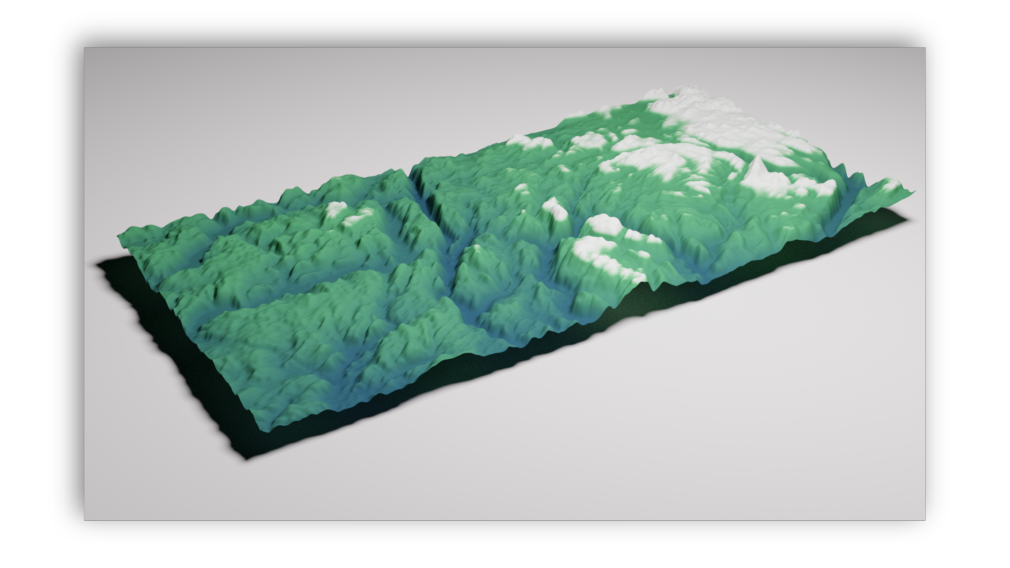
\includegraphics[width=1\linewidth]{images/terrain.pdf}
    \caption{Real terrain data from a region close to Stavanger, Norway. For
    the regression tasks, we select data from small rectangular regions to keep
    the data-sizes manageable. The data is supplied in the file
    \texttt{SRTM\_data\_1\_Norway.tif}.}
  \label{fig:terrain}
  \end{figure}

  The ordinary least squares and the Ridge regression is performed by solving
  the corresponding normal equations. We use the Lasso regression available in
  \textsc{sklearn} package.

  \section{Model statistics and resampling methods}
 	
  We are interested in computing certain statistical quantities pertaining to
  our data and corresponding model function. Firstly, the \emph{variance} of
  the model parameters \( \beta \) over all possible data sets tells us how
  sensitive \( \beta \) is to changes in the sampled data set. Using
  \cref{eq:optimal} for the optimal OLS-parameters and setting \( \mat{A} =
  (\X^T\X)^{-1}\X^T\), we compute:
  \begin{align}
	  \label{eq:ols_variance}
	  \cov\left[\beta_{\OLS}\right] &= \cov\left[\mat{A}\y\right] = \mat{A} \cov\left[\y\right] \mat{A}^T = \mat{A}\mat{A}^T\sigma^2 = (\X^T{\X})^{-1} \sigma^2.
  \end{align}
  In this calculation, we have used \cref{as:general_linear} to deduce that \(
  \cov[ \y ] = \diag{\sigma}\), a diagonal matrix, which commutes with other
  matrices. It then follows that the estimated variance of \( \beta_{\OLS} \) is given by
  \begin{equation}
	  \var[\beta_{\OLS}] = [\sigma^2 (\X^T\X)^{-1}_{ii} ]_{i=1}^n.
  \end{equation}
  Furthermore, by direct computation, we see that \( \beta_{\OLS} \) is an \emph{unbiased} estimator,
  as 
  \begin{equation}
	  \expect[\beta_{\OLS}] = \beta.
  \end{equation}
  With both the expected value and the variance of \( \beta \), we may
  formulate a confidence interval for \( \beta \). Thus for an estimated
  parameter \( \beta_i \) we construct the
  \(95\%\)-confidence interval as
  \begin{align}
	  \begin{split}
		  I_i &= (\expect[\beta_i] - 1.96 \times \SD[\beta_i], \expect[\beta_i] + 1.96 \times \SD[\beta_i]) \\
		      &= \left(\beta_i - 1.96 \times \sigma \sqrt{(\X^T\X)^{-1}_{ii}}, \beta_i + 1.96 \times \sigma \sqrt{(\X^T\X)^{-1}_{ii}}\right).
	  \end{split}
  \end{align}
  Here \( \SD[\beta_i] \) denotes the standard deviation of \( \beta_i \).  The
  interpretation of this interval is  ``under repeated experiments, the number
  of computed confidence intervals that actually include the true parameter,
  will tend to \( 95\% \)''.
 
  We are also interested in computing the model bias and variance as discussed
  in \cref{sub:bias_variance}. Numerically, we estimate these quantities by
  replacing the expectation values in \cref{eq:bias_variance} by averages.

  \subsection{Cross-validation}

  In order to obtain more reasonable estimates for these statistical
  quantities, we perform so-called \emph{resampling} of the data. There are
  several approaches to resampling, with two of the more common ones being
  \emph{bootstrap} and \emph{k-fold cross-validation}. Without going into
  details, the bootstrap method generally performs better with a significant
  data size, with cross-validation also performing well on smaller data sets.
  With this in mind, we will discuss cross-validation here.
  
  
  \chapter{Numerical Results}

  In this section we present some of the results of the numerical simulations.
  We start simple by first considering the effects of model complexity --- in
  terms of polynomial degree --- using OLS regression on the Franke dataset. We
  assess the model accuracy by means of the mean squared error and the \(
  R^2\)-score discussed previously. In order to increase the reliability of the
  statistical estimates, we employ \( k\)-fold cross validation.

  We then take a closer look at Ridge and Lasso regression techniques, and find
  the optimal hyper-parameter \( \lambda \). Again, we use the Franke dataset.
  In this context, we also see the effects of the bias-variance tradeoff.

  Finally, we compare our methods on real world data, namely the terrain data
  in \cref{fig:terrain}.
  
  \section{Toy Data}
  
  \begin{figure}
    \centering
    \subbottom{%
      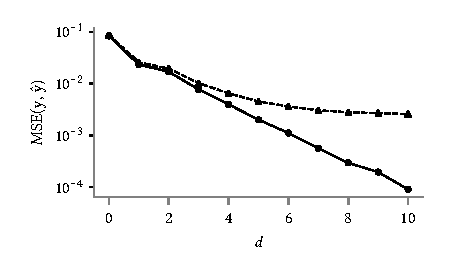
\includegraphics[width=0.45\linewidth]{images/OLS_MSE_score.pdf}
    }
    \subbottom{%
      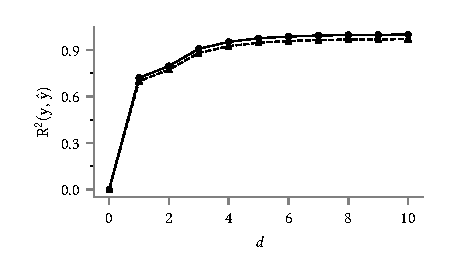
\includegraphics[width=0.45\linewidth]{images/OLS_R2_score.pdf}
    }
    \caption{Ordinary least squares regression on samples from the Franke
      function. The mean squared error (left) and the \(R^2\)-score (right) as
      a function of the polynomial degree \( d \). The values are displayed
      both for the true sample data (solid) and the noisy samples (dashed). The
      noise is distributed as \( \N(0, \tfrac{5}{100})\).}
    \label{fig:ols_scores}
  \end{figure}

\begin{figure}
    \centering
    \subbottom{%
      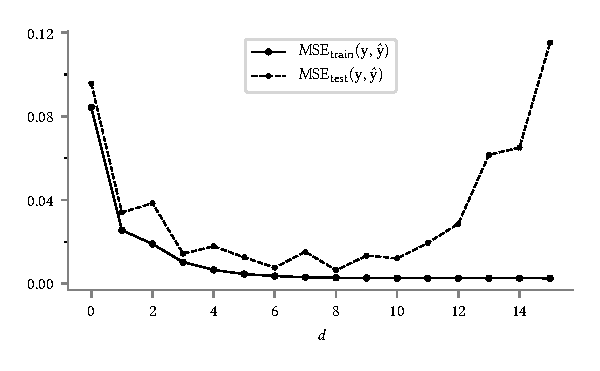
\includegraphics[width=0.45\linewidth]{images/OLS_MSE_score_crossval.pdf}
    }
    \subbottom{%
      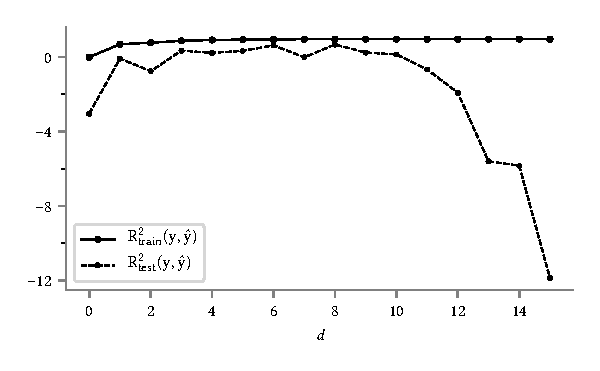
\includegraphics[width=0.45\linewidth]{images/OLS_R2_score_crossval.pdf}
    }
    \caption{Ordinary least squares regression on samples from the Franke
	    function with \( N = 100 \) points in each parameter direction,
	    yielding a total data-size of \( N^2 = 10000 \) points.  We have
	    used \( K \)-fold cross validation with \( K = 10 \).  The mean
	    squared error (left) and the \(R^2\)-score (right) as a function of
	    the polynomial degree \( d \). The values are displayed both for
	    the training data (solid) and the test data (dashed). The noise is
    distributed as \( \N(0, \tfrac{5}{100})\). Here we clearly see the effect
    of the bias-variance tradeoff. Note as the model complexity increases
    (higher polynomial degree), the model at some points overfits on the
    training data, yielding bad generalization scores, as signified by the
    sharp increase in \( \mathrm{MSE}_{\mathrm{test}} \).}
    \label{fig:ols_scores}
  \end{figure}

  \subsubsection{Ordinary Least Squares}
  
  We sample \( N = 1000 \) points in each parameter direction and compute the
  corresponding \( N^2 \) function values of the Franke function both with and
  without added noise. The noise was selected to be distributed as \( \N(0,
  1) \) with a signal-to-noise ratio \( \alpha = 0.05\).
  
  We then perform ordinary least squares, and compute the mean squared error as
  well as the \( R^2 \)-score for both the true and the noisy data. These are
  presented in \cref{fig:ols_scores}. With the Franke function being a weighted
  sum of exponentials, the MSE-error tends to zero as the polynomial degree
  increases. The added noise reduces the convergence rate, as is to be
  expected. 
  
  In addition to the evaluation metrics, we also compute confidence intervals
  for each model parameter. These are displayed in \cref{tab:ols_confidence}
  for each polynomial degree up to and including \( d = 5 \).
  
  \begin{table}
		\begin{tabular}{llllllr}
	\toprule
	{\(d\)} &    2 &         3 &         4 &         5 \\
	\midrule
	$1$       & \num{5.315e-05} & \num{6.349e-05} & \num{7.072e-05} & \num{6.696e-05} \\[1em]
	$x$       & \num{4.673e-04} & \num{1.682e-03} & \num{4.398e-03} & \num{8.402e-03} \\
	$y$       & \num{4.673e-04} & \num{1.683e-03} & \num{4.396e-03} & \num{8.400e-03} \\[1em]
	$x^2$     & \num{3.686e-04} & \num{6.458e-03} & \num{4.694e-02} & \num{1.959e-01} \\
	$x y$     & \num{2.948e-04} & \num{4.106e-03} & \num{2.873e-02} & \num{1.195e-01} \\
	$y^2$     & \num{3.686e-04} & \num{6.460e-03} & \num{4.692e-02} & \num{1.959e-01} \\[1em]
	$x^3$     &       {} & \num{2.575e-03} & \num{8.868e-02} & \num{9.884e-01} \\
	$x^2 y$   &       {} & \num{1.985e-03} & \num{5.199e-02} & \num{5.432e-01} \\
	$x y^2$   &       {} & \num{1.985e-03} & \num{5.199e-02} & \num{5.429e-01} \\
	$y^3$     &       {} & \num{2.575e-03} & \num{8.864e-02} & \num{9.884e-01} \\[1em]
	$x^4$     &       {} &       {} & \num{2.084e-02} & \num{1.078e+00} \\
	$x^3 y$   &       {} &       {} & \num{1.585e-02} & \num{6.287e-01} \\
	$x^2 y^2$ &       {} &       {} & \num{1.528e-02} & \num{5.443e-01} \\
	$x y^3$   &       {} &       {} & \num{1.585e-02} & \num{6.285e-01} \\
	$y^4$     &       {} &       {} & \num{2.083e-02} & \num{1.078e+00} \\[1em]
	$x^5$     &       {} &       {} &       {} & \num{1.658e-01} \\
	$x^4 y$   &       {} &       {} &       {} & \num{1.253e-01} \\
	$x^3 y^2$ &       {} &       {} &       {} & \num{1.193e-01} \\
	$x^2 y^3$ &       {} &       {} &       {} & \num{1.192e-01} \\
	$x y^4$   &       {} &       {} &       {} & \num{1.253e-01} \\
	$y^5$     &       {} &       {} &       {} & \num{1.658e-01} \\
	\bottomrule
	\end{tabular}
	\caption{The variance of the model parameters \( beta \) with respect
		to the polynomial degree \( d \). The corresponding basis
		function is displayed to the left. Note in particular how the
		variance of the model parameters seems to increase with the
		polynomial degree, which is what is to be expected according to
	the \emph{bias-variance tradeoff}.}
    \label{tab:ols_confidence}
  \end{table}

  \subsubsection{Ridge and Lasso regression}

  We now incorporate Ridge and Lasso regression in our numerical experiments.
  We are still working with the noisy sampled data.

  \section{Terrain Data}
	
  \chapter{Conclusion}

  
  \section{Further work}

  In this project we have discussed three different methods of linear
  regression.  In all three cases, we have fitted polynomial surfaces to the
  data sets. One draw-back with using polynomial surfaces is that they are
  inherently global methods. Thus, in order to capture local trends in the
  data, a very complex model is required, which (in the polynomial case) means
  surfaces of higher polynomial degree. In recent years, several attempts at
  constructing efficient local methods have been proposed. Spline-based
  (piecewise polynomial) methods in particular have been important, and several
  approaches to locally refined spline spaces have started to gain momentum.
  We note in particular that of \emph{hierarchical B-splines} (HB),
  \emph{truncated hierarchical B-splines} (THB) and \emph{locally refined
  B-splines} (LRB). These methods allow us to place more degrees of freedom in
  regions of high data-variance, thus locally increasing the model complexity.
  
  A study on least-squares surfaces using LR B-splines for representing terrain
  data was presented in \cite{skyttLocallyRefinedSpline2015}. Here, regions of
  high discrepancy between the true surface and the approximating surface was
  locally refined until an acceptable tolerance was reached.

  It would be interesting to make a comparison of the three methods in such a
  simple setting as linear regression, as done in this project, taking into
  account adaptive refinement of the spline spaces with respect to the sampled
  data set.
 

   

  \appendix
  \chapter{Derivation of the bias-variance-noise relationship}
  \label{ap:derivation}
  
  \if 0
  To this end --- by adding and subtracting \( f(\x_i) \) --- we have that 
  \begin{align}
    \begin{split}
      \expect_{\data, \varepsilon} \big[\cost(\data, \beta)\big] &= \frac{1}{n}\expect_{\data, \varepsilon} \left[\sum_{i = 1}^n (y_i - \hat{y}_i)^2\right] \\
                                                                 &= \frac{1}{n}\expect_{\data, \varepsilon} \left[\sum_{i=1}^n (y_i - f(\x_i) + f(\x_i) - \hat{y}_i)^2\right] \\
                                                                 &= \frac{1}{n}\sum_{i=1}^n\left\{\overbrace{\expect_{\varepsilon} \left[(y_i - f(\x_i))^2\right]}^{= \sigma^2} + \expect_{\data}\left[(f(\x_i) - \hat{y}_i)^2\right] + 2\overbrace{\expect_{\varepsilon}\left[y_i - f(\x_i)\right]}^{= 0}\expect_{\data}\left[f(\x_i) - \hat{y}_i\right] \right\} \\ 
                                                                 &= \frac{1}{n}\left\{n\sigma^2 + \expect_{\data} \left[(f(\x_i) - \hat{y}_i)^2\right]\right\} \\
                                                                 &= \sigma^2 + \frac{1}{n}\sum_{i=1}^n\expect_{\data} \left[(f(\x_i) - \hat{y}_i)^2\right]\right\}.
  \end{split}
  \end{align}

  Using the same trick of adding and subtracting, we may further decompose the second term as
  \begin{align}
    \begin{split}
      \expect_{\data} \big[ (f(\x_i) - \hat{y}_i)^2\big] = \left(f(\x_i) - \expect_{\data}\big[\hat{y_i}\big]\right)^2 + \expect_{\data} \left[\left(\hat{y}_i - \expect_{\data}\left[\hat{y}_i\right]\right)^2\right]
    \end{split}
  \end{align}
  \fi
  Combining the two previous equations, we obtain
 
\printbibliography
\end{document} 
